% Copyright (C) 2005-2015 Airbus - EDF - IMACS - Phimeca
% Permission is granted to copy, distribute and/or modify this document
% under the terms of the GNU Free Documentation License, Version 1.2
% or any later version published by the Free Software Foundation;
% with no Invariant Sections, no Front-Cover Texts, and no Back-Cover
% Texts.  A copy of the license is included in the section entitled "GNU
% Free Documentation License".
\renewcommand{\filename}{docUC_StocProc_StationaryCovarianceFunction_Estimation.tex}\renewcommand{\filetitle}{UC : Estimation of a stationary covariance function}

% \HeaderNNIILevel
%\HeaderIILevel
\HeaderIIILevel

\index{Stochastic Process!Stationary Covariance Function}

Let $X: \Omega \times \cD \rightarrow \Rset^d$  be a multivariate  stationary normal process of dimension $d$. We only treat here the case where the domain is of dimension 1: $\cD \in \Rset$ ($n=1$). \\
If the process is continuous, then $\cD=\Rset$. In the discrete case, $\cD$  is a lattice. \\

$X$ is supposed a second order process with zero mean. It is entirely defined  by  its covariance function $C^{stat}:  \cD \rightarrow  \mathcal{M}_{d \times d}(\Rset)$, defined by $C^{stat}(\tau)=\Expect{X_sX_{s+\tau}^t}$ for all $s\in \cD$.\\

In addition, we suppose that its spectral density function $S : \Rset \rightarrow \mathcal{H}^+(d)$ is defined,  where $\mathcal{H}^+(d) \in \mathcal{M}_d(\Cset)$ is the set of $d$-dimensional positive definite hermitian matrices.\\

The objective of this use case is to estimate $C^{stat}$ from a field or a sample of fields from the process $X$, using first the estimation of the spectral density function and then mapping $S$ into $C^{stat}$ using the inversion relation (\ref{cspectransform}), when it is possible.\\
As the mesh is a time grid ($n=1$), the fields can be interpreted as time series.\\

The estimation  algorithm is outlined hereafter.\\

Let $(t_{0},t_{1},\hdots t_{N-1})$ be the time grid on which the process is observed and let also $(\vect{X}^0, \dots, , \vect{X}^{M-1})$ be $M$ independent realizations of $X$ or $M$ segments of one realization of the process. \\
Using (\ref{cspectransform}), the covariance function writes:
\begin{equation}\label{TheoIntegral}
  C_{i,j}^{stat}(\tau)  = \int_{\mathbb{R}}\exp\left\{  2i\pi f \tau \right\} S_{i,j}(f)\, df
\end{equation}
where $C_{i,j}^{stat}$ is the element $(i,j)$ of the matrix $C^{stat}(\tau)$ and $S_{i,j}(f)$ the one of $S(f)$. The integral (\ref{TheoIntegral}) is approximated by its evaluation on the finite domain $\Omega \in \Rset$:
\begin{equation}\label{finiteApproximation}
  C_{i,j}^{stat}(\tau)  = \int_{\Omega}\exp\left\{  2i\pi f \tau \right\} S_{i,j}(f)\, df
\end{equation}
Let us consider the partition of the domain as follows:
\begin{itemize}
\item $\Omega =[-\Omega_c, \Omega_c]$ is subdivised into $M$ segments $\Omega$ = $\cup_{k=1}^{M} \mathcal{M}_k$ with $\mathcal{M}_k=[f_k - \frac{\Delta f}{2}, f_k + \frac{\Delta f}{2}]$
\item $\Delta f$ be the frequency step, $\Delta f = \frac{2 \Omega_c}{M}$
\item $f_k$ be the frequences on which the spectral density is computed, $f_k = -\Omega_c + \left(k - \frac{1}{2} \right) \Delta f = \left( 2 k - 1 - M \right) \frac{\Delta f}{2}$ with $k=1,2,\hdots,M$
\end{itemize}
The equation (\ref{finiteApproximation}) can be rewritten as:
\begin{equation*}
  C_{i,j}^{stat}(\tau)  = \sum_{k=1}^{M}\int_{\mathcal{M}_k}\exp\left\{  2i\pi f \tau \right\} S_{i,j}(f)\, df
\end{equation*}
We focus on the integral on each subdomain $\mathcal{M}_k$. Using numerical approximation, we have:
\begin{equation*}
  \int_{\mathcal{M}_k}\exp\left\{  2i\pi f \tau \right\} S_{i,j}(f)\, df \approx \Delta f S_{i,j}(f_k) \exp\left\{  2i\pi f_k \tau \right\}
\end{equation*}
$\tau$ must be in correspondance with frequency values with respect to the Shannon criteria. Thus the temporal domain of estimation is the following:
\begin{itemize}
\item $\Delta t$ is the time step, $\Delta t = \frac{1}{2 \Omega_c}$ such as $\Delta f \Delta t = \frac{1}{M}$
\item $\tilde{\mathcal{T}}$ =$[-T, T]$ is subdivised into $M$ segments $\tilde{{\mathcal{T}}}$ = $\cup_{m=1}^{M} \mathcal{T}_m$ with $\mathcal{T}_m=[t_m - \frac{\Delta t}{2}, t_m + \frac{\Delta t}{2}]$
\item $t_m$ be the time values on which the covariance is estimated, $t_m = -\frac{M}{2 \Omega_c} + \left(m - \frac{1}{2} \right) \Delta t = \left(2 m - 1 - M \right) \frac{\Delta t}{2}$
\end{itemize}
The estimate of the covariance value at time value $\tau_{m}$ depends on the quantities of form:
\begin{equation}\label{integral_subdomain_spectral}
  \int_{\mathcal{M}_k}\exp\left\{  2i\pi f \tau_{m} \right\} S_{i,j}(f)\, df \approx \Delta f S_{i,j}(f_k) \exp\left\{  2i\pi f_k \tau_{m} \right\}
\end{equation}

We develop the expression of $f_k$ and $\tau_{m}$ and we get:
\begin{equation*}
  \left\{
  \begin{array}{l}
    2m - 1 - M = 2 (m-1) - (M-1) \\
    2k - 1 - M = 2 (k-1) - (M-1)
  \end{array}
  \right.
\end{equation*}
Thus,
\begin{equation*}
  (2m - 1 - M) (2k - 1 - M) = 4 (m-1)(k-1) - (M-1)(2m -1 -M) - 2 (k-1)(M-1)
\end{equation*}
and :
\begin{equation*}
  (2m - 1 - M) (2k - 1 - M)\frac{\Delta t}{2}\frac{\Delta f}{2} = \frac{(m-1)(k-1)}{M} - \frac{(M-1)(2m -1 -M)}{4M} - \frac{(k-1)(M-1)}{2M}
\end{equation*}

We denote :
\begin{equation*}
  \left\{
  \begin{array}{l}
    \delta(m) = \exp\left\{-i \frac{\pi}{2M} (M-1)(2m -1 -M) \right\}\\
    \phi_k = \exp\left\{-i \frac{\pi}{M} (k-1)(M-1) \right\} S_{i,j}(f_k)
  \end{array}
  \right.
\end{equation*}

Finally, we get the followig expression for integral in (\ref{integral_subdomain_spectral})  :
\begin{equation*}
  \int_{\mathcal{M}_k}\exp\left\{  2i\pi f \tau_{m} \right\} S_{i,j}(f)\, df \approx \Delta f \exp\left\{2i \frac{\pi}{M} (m-1)(k-1)  \right\} \delta(m) \phi_k
\end{equation*}

It follows that :
\begin{equation}\label{expression_covariance_tm}
  C_{i,j}^{stat}(\tau_m)  = \Delta f \delta(m) \sum_{k=1}^{M} \phi_k * \exp\left\{2i \frac{\pi}{M} (m-1)(k-1)  \right\}
\end{equation}
In the equation (\ref{expression_covariance_tm}), we notice a discret inverse Fourier transform.\\ \\
OpenTURNS builds an estimation of the stationary covariance function on a \textit{ProcessSample} or \textit{TimeSeries} using the previous algorithm implemented in the \textit{StationaryCovarianceModelFactory} class. The result consists in a \textit{UserDefinedStationaryCovarianceModel} which is easy to manipulate. \\
Such an object is composed of a time grid and a collection of $K$ square matrices of dimension $d$. $K$ corresponds to the number of time steps of the final time grid on which the covariance is estimated.
When estimated from a time series , the \textit{UserDefinedStationaryCovarianceModel} may have a  time grid different from the initial time grid of the time series.\\



\requirements{

  \begin{description}
  \item[$\bullet$] a time series {\itshape myTimeSeries}
  \item[type:]  TimeSeries
  \end{description}

  \begin{description}
  \item[$\bullet$] a sample of time series {\itshape mySample}
  \item[type:]  ProcessSample
  \end{description}

  \begin{description}
  \item[$\bullet$] a spectral model factory {\itshape mySpectralFactory}
  \item[type:]  SpectralModelFactory
  \end{description}

}
{
  \begin{description}
  \item[$\bullet$] a factory {\itshape myFactory}
  \item[type:]  StationaryCovarianceModelFactory
  \end{description}

  \begin{description}
  \item[$\bullet$] a stationary covariance model: {\itshape myEstimatedModel\_TS, myEstimatedModel\_PS,}
  \item[type:]  UserDefinedStationaryCovarianceModel
  \end{description}
}

\textspace\\
Python script for this Use Case:

\inputscript{script_docUC_StocProc_StationaryCovarianceFunction_Estimation}



The following example illustrates the case where the avalaible data is a sample of $10^4$ realizations of the process, defined on the time grid $[0, 10]$, discretized every $\Delta t$ = $0.1$. The  covariance model  is the \textit{Exponential} model parametered by $\lambda = 1$ and $a = 1$, i.e.  $C^{stat}(\tau) = \exp(-|\tau|)$.\\

The Figure (\ref{StationaryCovarianceModelEstimation}) draws the graph of the exact covariance function and its estimation.
\begin{figure}[H]
  \begin{center}
    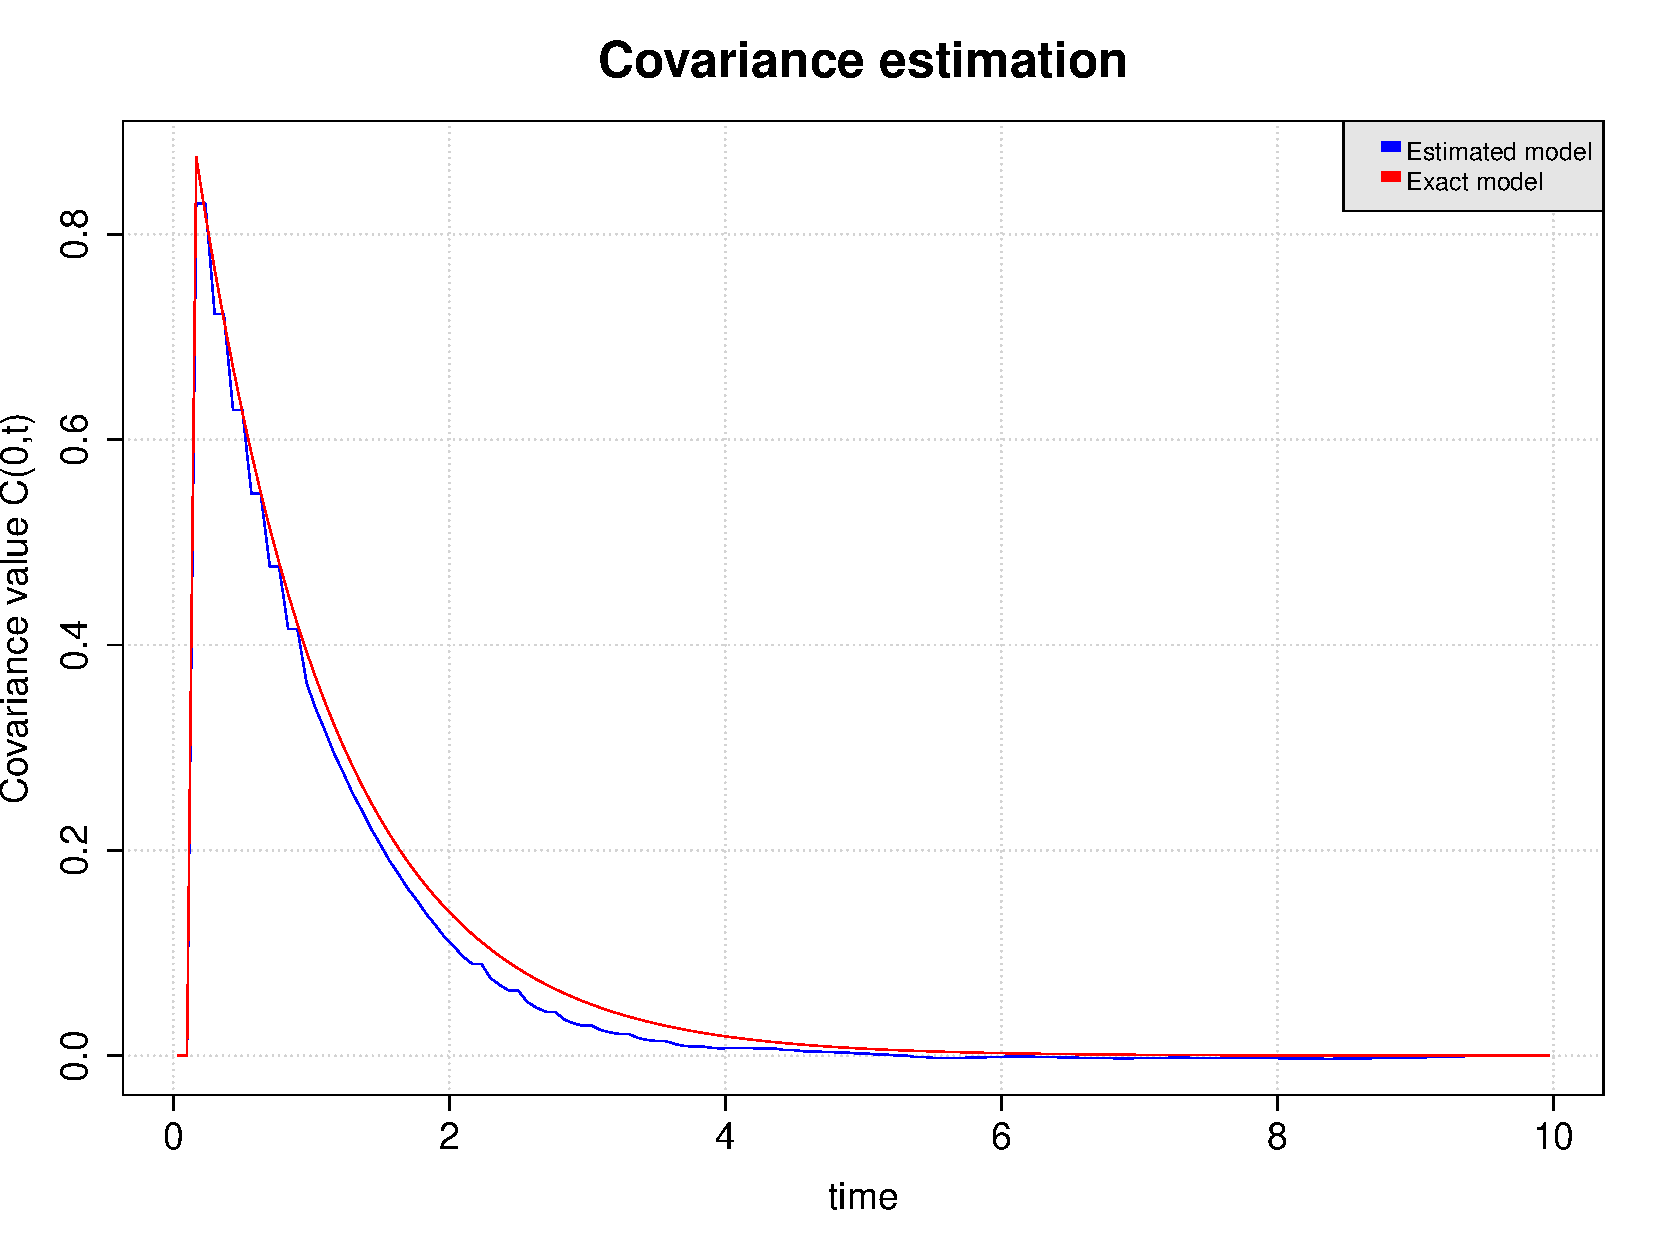
\includegraphics[width=7cm]{Figures/StationaryCovarianceModelEstimation.pdf}
    \caption{Covariance function $C(0,t)$ for $t$ in the time grid : estimation and exact model.}
    \label{StationaryCovarianceModelEstimation}
  \end{center}
\end{figure}
